\documentclass[10pt,twocolumn,letterpaper]{article}

\usepackage{../authorkit/cvpr}
\usepackage{times}
\usepackage{epsfig}
\usepackage{graphicx}
\usepackage{amsmath}
\usepackage{amssymb}

% Packages added by us
\usepackage{amsfonts}
\usepackage{mydefs}
\usepackage{algorithmic}
\usepackage{algorithm}

\usepackage[pagebackref=true,breaklinks=true,letterpaper=true,colorlinks,bookmarks=false]{hyperref}

% \cvprfinalcopy % *** Uncomment this line for the final submission

\def\cvprPaperID{****} % *** Enter the CVPR Paper ID here
\def\httilde{\mbox{\tt\raisebox{-.5ex}{\symbol{126}}}}

% Pages are numbered in submission mode, and unnumbered in camera-ready
\ifcvprfinal\pagestyle{empty}\fi
\begin{document}

%\title{Accelerating $\ell_1$-Minimization Using Many-Core CPUs/GPUs \\ and Application to Face Recognition
%\title{Efficient Parallelization of Sparse Representation for Face Recognition}
%\thanks{Corresponding author: . This work was partially supported by ARO MURI W911NF-06-1-0076.}}
\title{Efficient Parallelization of $\ell_1$-Minimization for Face Recognition
\thanks{Corresponding author: . This work was partially supported by ARO MURI W911NF-06-1-0076.}}

\author{First Author\\
Institution1\\
Institution1 address\\
{\tt\small firstauthor@i1.org}
% For a paper whose authors are all at the same institution,
% omit the following lines up until the closing ``}''.
% Additional authors and addresses can be added with ``\and'',
% just like the second author.
% To save space, use either the email address or home page, not both
\and
Second Author\\
Institution2\\
First line of institution2 address\\
{\small\url{http://www.author.org/~second}}
}

\maketitle

\begin{abstract}

\end{abstract}

\section{Introduction} 

%Motivate the paper by an overview about the scope and importance of $\ell_1$-minimization.
$\ell_1$-minimization is one of the most powerful tools to be added to the engineer's
toolbox in years.  It has strong theoretical motivation for both for use in recovering sparse
solutions to systems of linear equations, and has been shown to perform well even in the
presence of a combination of sparse and dense error.  Since solutions of linear systems
arise in practically every branch of engineering and there are very few application which
do {\em not} benefit from a robust error function, the applications are far to numerous to
itemize here.  
For many applications of $\ell_1$-minimization solving a system $b=Ax$, $A$ often has a
special structure that can be leveraged to compute portions of $A$ on the fly
as they are needed, speeding up perfomance of the minimization dramatically.
Unfortunately, there are many import applications where this does not hold true.
This paper targets applications where $\bb$ and $A$ contain
image data, and thus must be loaded every time they are used, as is the 
case for many problems in computer vision.
The techniques presented in this paper target these applications, as well
as others where the dictionary is dense and unstructured. $A$ must be loaded every time
it is used, and algorithm performance becomes highly dependent on memory bandwidth, rather
that arithmetic logic.

% Narrow focus for applications to Recognition Application
The primary motivating application for this paper is face recognition for access control applications.
Recently, advances in automatic face recognition have been made by re-casting
it as a sparse representation problem.  This core of this technique consists of
re-casting recognition as a sparse representation problem. This is done by  
stacking the test image into a vector $\bb$, stacking the training images for
all of the users into the columns of a matrix $A$, and solving the following
minimization problem:
\begin{equation}
\min_{\x, \e} \| \x \|_1 + \|\e\|_1 \quad \subj \quad \bb = A \x + \e.
\end{equation}
This optimization promotes a solution that is sparse both in $\x$ and $\e$. 
Sparsity in $\x$ arrises from the fact that only a subset of the training images (if any)
correspond to the user in the test image.  Sparsity in $\e$ arrises from the knowledge
that small occlusions in the test image will only corrupt a small subset of the pixels \cite{Wright2009-PAMI}.
The large coefficients in $\x$ will concentrate on the correct user, and can be used as the basis of a classifier.

For this idea to work, all of the images must be aligned. An iterative alignment
algorithm for this purpose was described as part of the \cite{Wagner2009-CVPR}, which was
the first paper to expand \cite{Wright2009-PAMI} into a functioning face recognition system.
This iterative alignment routine is based on repeatedly solving the following optimization problem:
\begin{equation}
\min_{\x, \e} \|\e\|_1 \quad \subj \quad \bb = A_k \x + \e.
\end{equation}
Where $A_k$ contains the training images for user $k$ as well as several vectors consisting of the
Jacobian of the test image $\bb$ with respect to the transformation parameters, and $\x$ contains
both the current representation coefficients, as well as an update to the transformation parameters.

\subsection{Literature review}
[Review the past parallel algorithms for $\ell_1$-minimization. Hopefully there aren't many]

[Review the available different algorithms solving $\ell_1$-minimization and $\ell_0$-minimization, please refer to Allen's SIAM paper.]
[Allen]

[Zero in and justify why we choose ALM for our implementation.]

\subsection{Contributions of the paper}

\section{Characteristics of the ALM Algorithm}
Describe the two variants of the ALM algorithm

The augmented lagrange multiplier (ALM) method utilizes a popular class of convex techniques, the lagrange multiplier, solving the problem:
\begin{equation}
F(x) = f(x) + \lambda g(x).
\end{equation}

Because the optimal lagrange multiplier values are not known, ALM iterates between estimating the solution and the lagrange multipier values.

In order to solve the recognition stage, we consider the $l_1$ problem:
\begin{equation}
\min_{\x, \e} \|\x\|_1 \quad \subj \quad \bb = A \x + \e.
\end{equation}
which can be formulated as
\begin{equation}
L_u(x,y) = \|x\|_1 + <\y, b - A\x - \e> + \frac{\mu}2 \| b-A\x-\e \|_2^2
\end{equation}

where $\mu > 0$ is a constant that penalizes infeasibility and $y$ is a vector of lagrange multipliers.

We summarize the entire ALM
algorithm as Algorithm~\ref{alg:alm}, where $\gamma$ denotes the
largest eigenvalue of the matrix $A^TA$. For the choice of parameter $\mu$, we take the same strategy as
in \cite{YangJ2009-pp} and set $\mu_0 = 2m / \|\bb\|_1$. We set $\rho=1.5$.
\begin{algorithm}[h]
\caption{\bf (Augmented Lagrange Multiplier Method Used in Alignment Inner Loop)}
\begin{algorithmic}[1]
\STATE {\bf Input:} $\bb \in \Re^m$, $A \in \Re^{m \times n}$,
$\x_1 = \mathbf{0}$, $\blamda_1 = \mathbf{0}$.
\WHILE{not converged ($k = 1,2,\ldots$)}
\WHILE{not converged ($l = 1,2,\ldots$)}
\STATE $\e_{l+1} \leftarrow \textup{shrink}\left(\bb - A\x_l + \frac{\blamda_k}{\mu_k}, \frac{1}{\mu_k}\right)$;
\STATE $\x_{l+1} \leftarrow (A^\dagger)^T \left(\bb - \e_{l+1} + \frac{\blamda_k}{\mu_k} \right) $;
\ENDWHILE
\STATE $\blamda_{k+1} \leftarrow \blamda_k + \mu (\bb - A\x_{k+1} - \e_{k+1})$;
\STATE $\mu_{k+1} \leftarrow \rho\mu_k$;
\ENDWHILE \STATE
{\bf Output:} $\x^* \leftarrow \x_k, \e^* \leftarrow \e_k$.
\end{algorithmic}
\label{alg:alm}
\end{algorithm}

In order to solve the alignment stage before recognition, we consider the $l_1$ problem: 
\begin{equation}
\min_{\x, \e} \|\e\|_1 \quad \subj \quad \bb = A \x + \e.
\end{equation}
which is solved in a similar fashion.

We need to define the following soft-thresholding operator for a
scalar $x$ and a scalar $\alpha \geq 0$:
\begin{equation}
\textup{shrink}(x,\alpha) = \textup{sign}(x)\cdot \max \{|x| - \alpha, 0\},
\end{equation}
In practice, this operator will be applied elementwise to a vector $\x$ with a single $\lambda$,
and will be notated as $\textup{shrink}(\x,\alpha)$.

Show Pseudocode for one variant
\subsection{Computational Complexity}
The Matrix-vector computions are O($mn$), and the vector-vector operations are O($m$), 
in terms of both computation cost and memory-bandwidth.
Therefore, assuming the iterative solver always takes a constant number of iterations,
the computational complexity of the overall algorithm is linear in the problem size.

\section{CPU Implementation}
% With a reshuffling of the order of operations and a change of the termination
% condition, the inner loop takes the form of two matrix-vector multiplications
% and a sequence of vector-vector operations.
\subsection{CPU Hardware Parallelism}
High-level discussion of CPU parallelism, i.e.
thread-level, vector-level, cache size, cache locality
\subsection{Tuning the GEMV operation}
When matrix-vector operations are called sequentially on the same data,
the operation can be blocked so that each thread operates on the same block of data for each operation.

For Single threaded MKL sgemv, Code took          0.0335823 msec per instance to run!

For Automatic multi-threaded MKL sgemv, Code took 0.008179 msec per instance to run!

For Manually multi-threaded MKL sgemv, Code took  0.0061276 msec per instance to run!

\subsection{Tuning the Soft-Thresholding Operator}
...Make sure there are no branches

...Make sure there are no function calls

...Make sure the loop gets automatically vectorized

...Block the computation into work for different cpu cores

\section{GPU Implementation}
\subsection{GPU Hardware Parallelism}
High-level description of GPU parallelism, i.e.

The ALM algorithm requires many matrix-vector operations, this gives manycore processors such as GPUs a computational advantage for large problem sizes.  
GPUs are comprised of several streaming multiprocessors, which contain 32 floating-point units.  The GPU executes programs as SIMT (Single Instruction Multiple Threads) in groups of 32 threads called warps.  These warps are then grouped into higher levels called thread blocks and grids.  The improvement in speed comes from the memory structure of the GPU.   The GPU contains an inverted memory hierarchy so that the L2 cache stays close to the cores, providing the increase in performance.  It essentially turns the GPU from being memory-limited to computational-limited.
GPU memory also differs from CPU memory in that it requires data transfers over PCI-Express.  The cost of these transfers are amortized by doing large amounts of computation at once, requiring code to be run completely on the GPU.  The GPU can be analogous to a multi-core CPU processor, except with more sophisticated vector processing hardware.  Each streaming multiprocessor is analogous to a single CPU except that it can run multiple threads simultaneously... 


%You should give a brief (1-2 paragraphs) overview of the GPU architecture -- most people have heard of GPUs and what they can do by now, so it isn't worth spending a whole lot of space in the paper describing it.

%You should define the levels of the Cuda thread and memory hierarchies: i.e. warps, thread blocks, grids and register file, shared memory, global memory. Also mention that the GPU memories are all distinct from the CPU memories, and data transfers go over PCI-Express -- but the cost of those transfers are amortized by doing lots of work (i.e. solving an l1 minimization after transferring the matrix once). It is worth spending a little space describing how the GPU is a multi-core processor (just like the CPUs), but with much more sophisticated vector processing hardware. That is: on a Fermi there are 15 cores, and each one has two 16-wide vector floating-point units.

%The GPU-algorithm is the same as the CPU algorithm: primary- and dual- ALM methods. The implementations differ in that you have to parallelize the GPU code at an additional level, and you can't use the GPU's caches to communicate between cores (only within a core). On the CPU, you only need to parallelize for the 4 or 8 cores -- and perhaps add SSE instructions when possible (usually this is inside of the BLAS library) -- any communication between cores happens implicitly via cache coherence. For the GPU, you need to parallelize for the 15 cores, but also for the 32-way SIMD parallelism of Warps. Any intra-core communication happens via the cache (aka scratchpad, or __shared__ memory) and within-block barriers (i.e. __syncthreads()), and any inter-core communication happens via the GPU's DRAM and the implicit barriers between grid launches.


cuda cores, SIMD width, scheduling restrictions, bandwidth
\subsection{Solving a Single L1 minimization}
This section is about Victor's CUBLAS implementations.
Plot Solver Bandwidth in GB/s vs. Problem size in MB

The GPU ALM algorithm is written in CUDA and utilizes the CUBLAS libraries.  The algorithm is the same as the CPU algorithm except that we had to parallelize the GPU at an additional level.  The CPU portion of the code acts as a conductor, making calls to GPU functions in C, while the GPU portion does the computation.

\subsection{Solving multiple L1 minimizations in parallel}
This section is about Drew's kernels for solving multiple L1 minimizations in parllel

How to efficiently perform an L1 minimization on a single core, quote performance on a large batch.

How to solve multiple instances in smaller batches without losing concurrency, using CUDA streams.

...Mention effect of compiler verion on streams implementation

\section{Benchmarks on Synthetic Data}
\subsection{PALM L1 minimization benchmark}

In this section, we benchmark the performance of MATLAB, BLAS MKL, and GPU Cuda implementations of the Primal ALM algorithm on synthetic data to find the point at which the GPU version runs faster than CPU versions.
To simply the benchmark, we cap the number of inner iterations at 50 and outer iterations at 5000 and run the algorithm to convergence.
CPU code was run on an Intel Dual Socket Quad Core with 8 gigs of DDR3 RAM.  GPU code was run on a GTX480
We ran the A matrix with different ratios between m:n from 10:1:5 for m:2000:25:8000 with an x vector of 10 percent sparsity.  Tolerance levels were empirically seen to allow best performance with the inner loop tolerance set at one order of magnitude lower than the outer loop tolerance.

%An example of image inclusion for Victor:
\begin{figure*}
\centering
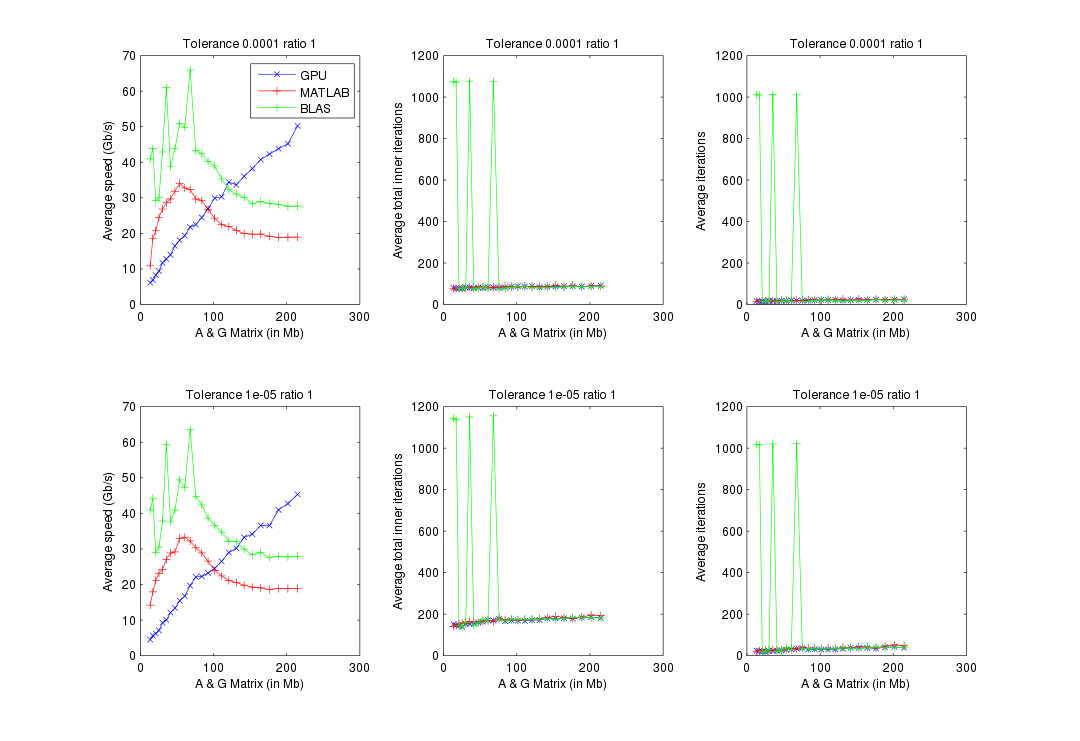
\includegraphics[width=3.5in]{figures/PALM_benchmark_ratio_1.png}
\caption{This is where the caption goes.}
\label{fig:uniqueidentifierforthisimage}
\end{figure*}

As the dimensions of A increase, so does the significance of the size of AtA.  Until the A and AtA matrix reach x Mb, the CPU version runs faster than the GPU.  

Optimization:
\begin{equation}
\min_{\x, \e} \|\x\|_1 \quad \subj \quad \bb = A \x + \e.
\end{equation}

$A$ is $m \times n$
$m = 5120$
$n = 32$

One of these minimizations is performed per 
alignment iteration in our face recognition pipeline.

All of the following are implementations of primal ALM.
Primal ALM contains outer and inner iterations.
To simplify the benchmark, the number of outer iterations
is clamped to 50, and the number of inner iterations is
clamped to 50 iterations per outer loopsretrsitrsi.  Running with
a convergence criterion will typically result in fewer
iterations, depending on the data, so these numbers are
for comparison across hardware, and may look worse than
with other benchmarks on face data.

To generate a meaningful comparison between different hardware
architectures, we compare on a per-board basis:

For CPU implementations, the benchmark makes use of
as all of the cores in as many cpu's are present.

For GPU implementations, the benchmark makes the best use
of the entire GPU chip (most GPU boards have a single GPU chip).

Since different platforms may perform most efficiently when
executing multiple L1 minimizations simultaneously,
we quote the average time required to solve a single L1
minimization problem instance.

schur:  Mac Pro, dual socket, quad core, hyperthreading intel nehalem @ 2.66 GHz

Nvidia GTX480: This is the current state of the art consumer card.  
It is clocked slightly faster than the pro version of the card, so it 
should have slightly faster single precision float performance. (double precision is crippled, though)
GTX480 has 15 cores, each of which has 2x32-wide floating point pipelines.
All Fermi GPU's have 768KB L2 cache.

Zihan's OpenCV implementation: *** 190 ms per L1 minimization ***
amortized over 16 instances,
four of which run simultaneously.  Tuning note:  the cpus
can support up to 16 logical threads, but 4 instances seem
sufficient to saturate the memory architecture.  Using more
than 5 instances results in lower performance, perhaps due
to less efficient usage of the cpu caches.

Zihan's MATLAB implementation: *** 60 ms per L1 minimization ***
This is amortized over 100 sequential instances.  All 16 logical
cores were used, i.e. showed 100% usage in htop.  Pararllelism
is a result of MATLAB's usage of Intel's MKL, a parallel blas
implementation. I believe performance is very high to
efficient cache usage:

The A matrix takes up 5120*32*8 bytes = 1.25 MB
The two processors have 16MB L3 Cache in total.
The two processors have 2MB L2 Cache in total.

Drew's pure CUDA, single kernel implementation: *** 36 ms per L1 minimization ***
This implementation performs L1 minimization on 60 instances of L1.
They are all run as a single cuda kernel.  
Each instance of L1 is mapped onto a cuda block. (tuned to 64 threads / block)
This means that the GPU hardware will schedule the multiple instances to run
on the (15 for GTX480) cuda cores as concurrently (15? 30?) as possible.  
For this to work, all of the data has to be ready at the same time.

Drew's pure CUDA, streams implementation: *** 70 ms per L1 minimization ***
This implementation performs L1 minimization on 60 instances of L1.
Each instance of L1 is mapped onto a cuda block. (tuned to 128 threads / block)
Each instance is run in a separate single-block CUDA kernel.
The 60 kernels are added to 15 cuda streams.
The GPU (hardware? driver?) then runs the kernels, up to 15 concurrently.

Victor's CUDA/cublas mixed implementation: *** 302 ms per L1 minimization ***
This implementation makes use of hand-written kernels for vector-vector operations,
and cublas for matrix-vector operations.  There are two implementations under development:
1. Perform a single L1 minimization using the entire GPU.
2. Use cuda streams to perform multiple L1 minimizations concurrently on the GPU.
Benchmarked on Drew's GTX480

Drew's OpenMP implementation: *** 200 ms per L1 minimization***
Benchmarked on schur(Dual Socket Quad Core Nehalem), all compiler optimizations turned on.
This divides the matrix operations into 8 chunks, each of which is handled by a thread
on a different CPU core.  Fine-grained parallelism is achieved through SSE2 vector
floating point operations.  This implementation should ultimately beat the MATLAB/MKL
implementation, especially for small problem sizes, since the primary advantage
over MKL is a reduction in the number of times image-sized temporary variables
are written and read from memory. 

Drew's Single-Threaded MKL implementation: *** 226 ms per L1 minimization ***
Benchmarked on schur(Dual Socket Quad Core Nehalem), all compiler optimizations turned on.
Uses MKL for single-threaded matrix-vector multiplies.  
Saves ~almost as many writes of temporary vector variables as the previous OpenMP implementation.
Shrinkage operator improved; at least with g++ there is now no branching or function call overhead.
This implementation uses a single CPU core...
... so if linear speedup can be achieved, could possibly get *** 28 ms per minimization ***




%\begin{algorithm}[thb]
%\caption{\bf (Deformable Sparse Recovery and Classification for
%Face Recognition)} \label{alg:deformable-src}
%\begin{algorithmic}[1]
%\STATE {\bf Input:} Frontal training images $A_i \in \Re^{m\times n_i}, i=1,2,\ldots,K$ for $K$ subjects,  a test image
%$\bb\in\Re^m$ and a deformation group $T$. 
%\STATE
%{\bf for} each subject $i$, 
%\STATE \hspace{3mm} $\tau^{(0)}
%\leftarrow I$. 
%\STATE \hspace{3mm} {\bf while} not converged $(j=1,2,\ldots)$ {\bf do} 
%\STATE \hspace{6mm}
%$\tilde \bb(\tau) \leftarrow \frac{\bb \circ \tau}{\|\bb \circ
%\tau\|_2}$; \;\;\; $J \leftarrow  \frac{\partial}{\partial
%\tau} \tilde\bb(\tau)  \bigr|_{\tau^{(j)}} $;
%%\STATE \hspace{6mm} $(\hat \x, \hat \e, \Delta \tau) \leftarrow \left\{\begin{array}{l} \arg \min_{\x,\e,\Delta \tau} \| \e \|_1 \\  \subj \; \bb + J \Delta \tau = A_k \x + \e \end{array}\right.$
%\STATE \hspace{6mm} $ \Delta \tau =  \arg\min \; \| \e \|_1  \;
%\subj \; \tilde \bb + J \Delta \tau = A_i \x + \e.$ 
%\STATE
%\hspace{6mm} $\tau^{(j+1)} \leftarrow \tau^{(j)} + \Delta
%\tau$; 
%\STATE \hspace{3mm} {\bf end while} \STATE {\bf end} \STATE Keep
%the top $S$ candidates $k_1, \ldots, k_S$ with the smallest
%residuals $\|\e\|_1$. \STATE Compute an average transformation
%$\bar{\tau}$ from $\tau_{k_1}, \tau_{k_2}, \ldots, \tau_{k_S}$.
%\STATE Update $\bb \leftarrow \bb \circ \bar{\tau}$ and $\tau_i
%\leftarrow \tau_i \cdot \bar{\tau}^{-1}$ for $i = k_1, \dots,
%k_S$. \STATE Set $A \leftarrow \big[ A_{k_1} \circ
%\tau_{k_1}^{-1} \mid A_{k_2} \circ \tau_{k_2}^{-1} \mid \dots
%\mid A_{k_S} \circ \tau_{k_S}^{-1} \big]$. \STATE Solve the
%$\ell^1$-minimization problem:
%$$\hat{\x} = \arg \min_{\x, \e} \| \x \|_1 + \|\e\|_1 \;\; \subj \;\; \bb = A \x + \e.$$
%\STATE Compute residuals $r_i(\bb) = \| {\bb} - {A}_i \, \delta_i(\hat{\x}) \|_2$ for $i = k_1, \dots, k_S$.
%\STATE {\bf Output:} $\mbox{identity}(\bb) = \arg\min_i r_i(\bb)$.
%\end{algorithmic}
%\end{algorithm}

%We summarize the entire ALM
%algorithm as Algorithm~\ref{alg:alm}, where $\gamma$ denotes the
%largest eigenvalue of the matrix $A^TA$. For the choice of parameter $\mu$, we take the same strategy as
%in \cite{YangJ2009-pp} and set $\mu = 2m / \|\bb\|_1$.
%\begin{algorithm}[h]
%\caption{\bf (Augmented Lagrange Multiplier Method for Global
%Recognition)}
%\begin{algorithmic}[1]
%\STATE {\bf Input:} $\bb \in \Re^m$, $A \in \Re^{m \times n}$,
%$\x_1 = \mathbf{0}$, $\e_1 = \bb$, $\blamda_1 =
%\mathbf{0}$.
%\WHILE{not converged ($k = 1,2,\ldots$)}
%\STATE $\e_{k+1} = \textup{shrink}\left(\bb - A\x_k +
%\frac{1}{\mu}\blamda_k, \frac{1}{\mu}\right)$;
%\STATE $t_1\leftarrow 1$, $\z_1 \leftarrow \x_k$, $\w_1 \leftarrow \x_k$;
%\WHILE{not converged ($l = 1,2,\ldots$)}
%\STATE $\w_{l+1} \leftarrow \textup{shrink}\left(\z_l +
%\frac{1}{\gamma}A^T\left(\bb - A\z_l - \e_{k+1} +
%\frac{1}{\mu}\blamda_k\right), \frac{1}{\mu\gamma}\right)$;
%\STATE $t_{l+1} \leftarrow \frac{1}{2}\left( 1 +
%\sqrt{1+4t_l^2}\right)$;
%\STATE $\z_{l+1} \leftarrow \w_{l+1} + \frac{t_l - 1}{t_{l+1}}(\w_{l+1} - \w_l)$;
%\ENDWHILE
%\STATE $\x_{k+1} \leftarrow \w_{l}$;
%\STATE $\blamda_{k+1} \leftarrow \blamda_k + \mu (\bb - A\x_{k+1} - \e_{k+1})$;
%\ENDWHILE \STATE
%{\bf Output:} $\x^* \leftarrow \x_k, \e^* \leftarrow \e_k$.
%\end{algorithmic}
%\label{alg:alm}
%\end{algorithm}


\section{Conclusion}
...How lessons from this paper extend (or don't extend) to other similar problems in computer vision

...Reiterate how the appropriate hardware choice depends on the problem size.

{\small
\bibliographystyle{../authorkit/ieee}
\bibliography{faces}
}


\end{document}
